\section{Gabriel Development Tool for Object Detection}

Existing ad-hoc approach to develop wearable cognitive assistance not only takes
a long time, but also requires computer vision expertise. A developer new to
wearable cognitive assistance would need to spend months learning computer
vision basics and acquire intuitions to determine what is achievable before
developing an application. For instance, a researcher mentions the first
application developed to help a user assemble LEGO pieces took him more than
four months.

%% \begin{figure}
%% \centering
%% 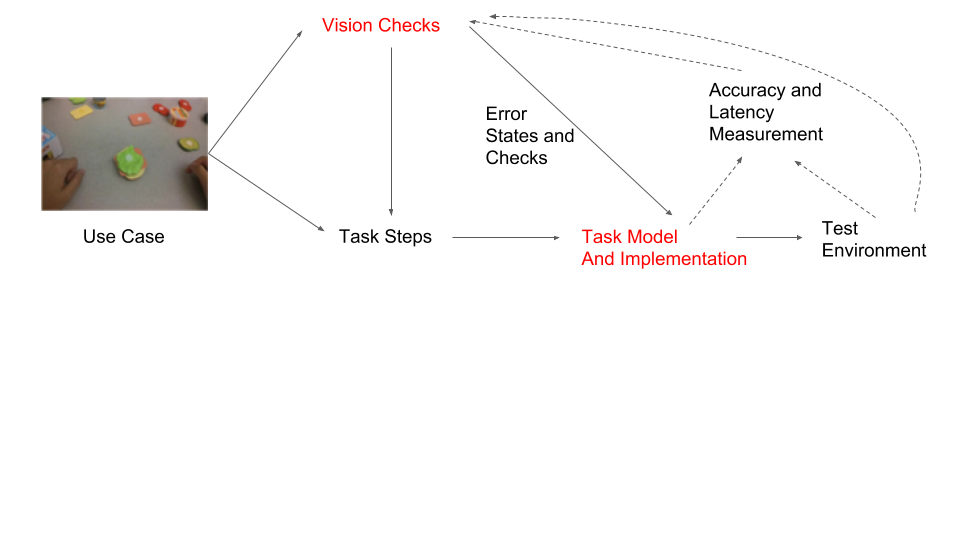
\includegraphics[trim={0 3in 0 0.2in},clip,width=7in]{FIGS/ad-hoc-workflow}
%% \caption{Ad-hoc Existing Workflow}
%% \label{fig:adhoc-workflow}
%% \end{figure}

Figure~\ref{fig:workflow} shows the ad-hoc development process. The most
critical step in building wearable cognitive assistance is to identify task
steps and the visual states of task steps. For example, for the Lego wearable
cognitive assistance ~\cite{chen2017empirical}, the task steps are the sequence
of shapes needed to achieve the final assembled lego shape. The visual states to
recognize are the current shapes on the lego board. Identifying visual states
and task steps takes significant time and expertise due to several reasons.
First, a developer needs to be familiar with the state-of-art of computer vision
algorithms to determine what visual states can be recognized reliably. Second,
identifying task steps requires domain knowledge. Third, when visual states
become too hard for CV, developers need to adjust the task steps to use other
methods for confirmation. Often a redesign of task steps is required to
compensate computer vision. For instance, when designing the RibLoc application,
a redesign of the task steps involves asking the user to read out a word on the
gauge instead of performing optical character recognition on the lightly-colored
characters.

I plan to work on building Gabriel development tools in my thesis. I want to
focus on providing automation tools for the most time-consuming procedures in
the development workflow -- building vision checks.

%% Object detection is at the core of computer vision tasks used by Gabriel
%% application. In Ping-Pong assistance, the Ping-Pong table, the ball, and the
%% opponent need to be recognized and localized. In Ikea Lamp assistance, the lamp
%% base, the shade, and the bulb need to be detected. Being able to create reliable
%% object detectors quickly can substantially facilitate application development.

%% Recent advances in
%% DNNs~\cite{girshick2014rich},~\cite{ren2015faster},~\cite{he2016deep} have not
%% only drastically improved the accuracy of object detection, but also provide an
%% opportunity to automate the creation of them. Unlike traditional CV algorithms,
%% DNNs adopt a end-to-end learning approach, in which features are no longer
%% hand-crafted but learned. The replacement of custom CV code with machine-learned
%% models gives automation opportunities. Nevertheless, creating a DNN-based object
%% detector is still both time-consuming and painstaking due to other reasons. DNNs
%% have a lot of parameters and requires millions of labeled examples to train from
%% scratch. Collecting and labeling these large amount of training data becomes a
%% bottleneck.

TPOD (Tool for Painless Object Detection) is a web-based tool I developed to
help quickly create DNN-based object detectors. It provides a tracking-assisted
labeling interface for speedy labeling and transfer learning-based DNN training
and evaluation backends that abstract the nuances of DNNs. Using TPOD to create
object detectors is straight-forward. A user would first upload short videos of
the object collected from varying lighting conditions and perspectives. Then,
the user would label these objects using TPOD's labeling interface. TPOD assists
labeling by tracking the labeled object across frames. Augmenting training data
with synthetically generated data is also supported. A user then can start training
from the web interface. TPOD backend uses transfer learning to finetune an
object detector DNN from publicly available networks that have been trained with
millions of images. When the training is done, a user can download the object
detector as a container image to run the trained models for inference. TPOD also
provides interfaces for evaluating and testing trained DNNs.

The initial prototype of TPOD has been used by researchers and students to build
wearable cognitive assistance. For example, a group of master students in CMU
mobile and pervasive computing class successfully used TPOD to build an
assistant for using AED machines.

Going forward, I plan to open-source the tool after following optimizations.
First, TPOD's backend needs to be easily extensible. With increasingly many
DNN-based object detectors developed in the computer vision community, adding a
new object detector to TPOD should be made easy. This design goal requires
well-modularized DNN backends with clean and easy-to-use interfaces to query
labeled datasets for training, standard serialization format to download, and
stable APIs to detect objects using the trained models. Second, TPOD's labeling
interface should be well isolated from the automated DNN training backend. With
such isolation, individuals looking for labeling tools can leverage TPOD's
front-end without setting up the training backend. This isolation requires
serializing labeled datasets using widely-used formats, for example, Pascal VOC
annotation format. Third, TPOD should be packaged well for installation. I plan
to containerize TPOD to make it easy for others to install.

\clearpage

%% \subsection{Automatic Workflow Extraction}

%% Identifying and implementing the task model in a wearble cognitive assistance
%% also takes a considerable amount time. In existing workflow, both these steps
%% are done manually with developers' domain knowledge, experience and intuition.
%% Automatic extraction of a workflow and generation of the task model
%% implementation can greatly reduce the development time.

%% Particularly, I will focus on mechanical assembly tasks since they often have
%% non-trivial number of steps and complex task model. I plan to work on automatic
%% extraction of workflow from videos. The inputs are videos recordings of correct
%% assembly procedures. The outputs are step sequences annotated with objects
%% involved for each step. Once the task model is extracted, a developer is able to
%% edit and add error states to complete the task model. In addition, I will strive
%% for building tools to generate code blocks from a task model.
